\documentclass{templateNote}
\usepackage{tcolorbox}
\usepackage{hyperref}
% \usepackage{pgfplots}
\usepackage{amsmath}
\usepackage{amssymb}

\begin{document}

\imagenlogoU{img/logoNGMFormal_sinF.png}
\linklogoU{https://github.com/NicoxlkboUni} 
% \imagenlogoD{img/logo-ubb-txt-face.png} 
% \linkQRDoc{https://github.com/NicoxlkboUni} %TODO: Eliminar este qr
\titulo{Unidad 1}
\asignatura{Gestión Estrategica}
\autor{
    \indent
    Nicolás \textsc{Gómez Morgado}
}

\portada
\margenes % Crear márgenes
\tableofcontents
\newpage

\section{Conceptos a tener en cuenta}
\begin{itemize}
    \item Estado $\neq$ Gobierno.
    \item Estado: Conjunto de personas que habitan el país.
    \item Gobierno: Administración del Estado.
    \item Estado de derecho: Las decisiones son tomadas por el congreso. 
\end{itemize}

\section{Tipos de Organizaciones:}
\begin{itemize}
    \item Según lo que produce:
        \begin{itemize}
            \item Primarias
            \item Secundarias
            \item Terciarias
        \end{itemize}
    \item Según actividad desarrollada:
        \begin{itemize}
            \item Agropecuarias
            \item Mineras
            \item Manufactureras
            \item Servicios (Universidades por ejemplo)
        \end{itemize}
    \item Según su fin:
        \begin{itemize}
            \item Con fines de lucro
            \item Sin fines de lucro (Sus fondos se invierten en la organización)
            \begin{itemize}
                \item Fundaciones
                \item Corporaciones
            \end{itemize}
        \end{itemize}
    \item Según tipos de bienes que produce:
        \begin{itemize}
            \item Consumo final
            \item Bienes Intermedios
        \end{itemize}
    \item Según formas de producción:
        \begin{itemize}
            \item Artesanal (Trabajo manual)
            \item Tecnología media
            \item Alta tecnología
        \end{itemize}
    \item Según quien la dirige o decide:
        \begin{itemize}
            \item Autogestiones (Jefe es la autoridad total)
            \item Heterogestionada (Multitud de jefes a través de acciones)
            \item Cogestionada (Decisiones tomadas por jefe y gerente/s)
        \end{itemize}
    \item Según su localización:
        \begin{itemize}
            \item Local (Empresa con ubicación única)
            \item Nacional (Empresa con multiples ubicaciones en el país)
            \item Internacional (Empresa con ubicaciones en varios países)
        \end{itemize}
    \item Según forma de gestión;
        \begin{itemize}
            \item Centralizada (Manejo general)
            \item Descentralizada (Manejo individual por sucursal)
        \end{itemize}
    \item Según propiedad o aportes de capital:
        \begin{itemize}
            \item De personas
                \begin{itemize}
                    \item Responsabilidad limitada
                    \item Responsabilidad ilimitada
                \end{itemize}
            \item De capital
                \begin{itemize}
                    \item Sociedad anónima cerrada
                    \item Sociedad anónima abierta
                \end{itemize}
            \item Mixta o comandita
            \item Cooperativa
            \item Publicas
        \end{itemize}
    \item Según tamaño y estructura:
        \begin{itemize}
            \item Artesanal (1-9 trabajadores)
            \item Pequeña empresa (19-49 trabajadores)
            \item Mediana empresa (50-199 trabajadores)
            \item Gran empresa (200 o más trabajadores)
        \end{itemize}
    \item Según nivel de ventas:
        \begin{itemize}
            \item Microempresa (Hasta 1000 UF)
            \item Pequeña empresa (Hasta 25000 UF)
            \item Mediana empresa (Hasta 100000 UF)
            \item Gran empresa (Más de 100000 UF)
        \end{itemize}
    \item Según estructura:
        \begin{itemize}
            \item Formal (Planificación y estructura jerárquica)
            \item Informal (Nace de forma espontanea por afición de personas e intereses comunes)   
        \end{itemize}
\end{itemize}

\section{Procesos de Administración Estratégica}
\begin{itemize}
    \item Selección de la misión y objetivos
    \item Análisis del entorno competitivo externo (Oportunidades y Amenazas)       
    \item Análisis del entorno competitivo interno (Fortalezas y Debilidades)
    \item Formulación de estrategias (Decidir el camino de la empresa)
    \item Implementación de estrategias (Como y quien hace las cosas)
    \item Control de estrategia (Chequeo antes, durante y después del proceso)
\end{itemize}

\section{Fuerzas que mueven a la competencia}
\begin{itemize}
    \item \textbf{Las 5 fuerzas de Porter}
    \begin{itemize}
        \item Amenaza ingreso de nuevos competidores potenciales (ANE)
        \item Amenaza de productos sustitutos (APS)
        \item Rivalidad competidores existentes (RC)
        \item Poder negociador de los clientes (PNC)
        \item Poder negociador de los proveedores (PNP)
    \end{itemize}
\end{itemize}

\section{Herramientas de análisis}
\subsection{Análisis competitivo}
    \begin{itemize}
        \item \textbf{Análisis FODA}
        \begin{itemize}
            \item \textbf{Fortalezas:} Ventajas con respecto a otras empresas las cuales mejoro o potencio.
            \item \textbf{Oportunidades:} Situaciones que ofrece el entorno en las cuales la empresa puede obtener algún tipo de beneficio.
            \item \textbf{Debilidades:} Implican costos o resultados negativos en su entorno, se buscan minimizar o eliminar.
            \item \textbf{Amenazas:} Situaciones presentes en el entorno que pueden afectar negativamente a la empresa, ante las cuales se prevenga o prepare.
        \end{itemize}
    \end{itemize}

\subsection{Análisis de cartera de actividades}
    \begin{itemize}
        \item \textbf{Matriz BCG} (Boston Consulting Group)
        \begin{itemize}
            \item \textbf{Estrellas:} Productos con alta participación en el mercado y alto crecimiento. \textbf{(Relevar a las vacas lecheras)}
            \item \textbf{Interrogantes:} Productos con baja participación en el mercado y alto crecimiento. \textbf{(Desarrollarse o retirarse)}
            \item \textbf{Vacas lecheras:} Productos con alta participación en el mercado y bajo crecimiento. \textbf{(Cosechar utilidades)}
            \item \textbf{Perros:} Productos con baja participación en el mercado y bajo crecimiento. \textbf{(Retirarse o sobrevivir)}
        \end{itemize}
        \begin{figure}[H]
            \centering
            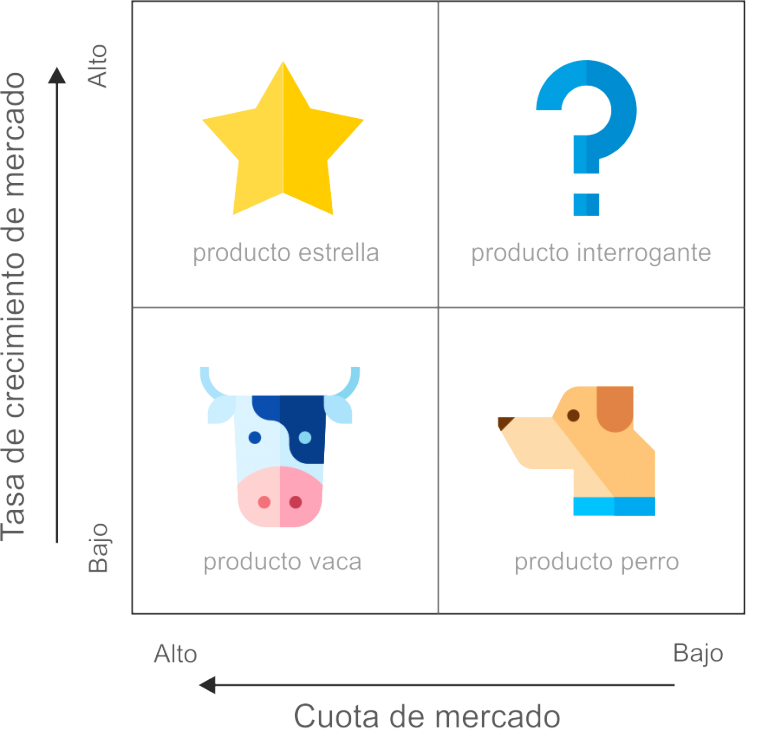
\includegraphics[width=0.5\textwidth]{img/matriz_bcg-768x803.png}
        \end{figure}
        \item \textbf{Matrices de Planificación}
        \begin{itemize}
            \item \textbf{Matriz de crecimiento-participación:} Analizar como funcionaria nuestra empresa en el mercado.
            \item \textbf{Matriz atractivo de la industria-fortaleza del negocio:} Analizar la industria, ver competencia y ventaja competitiva.
            \begin{figure}[H]
                \centering
                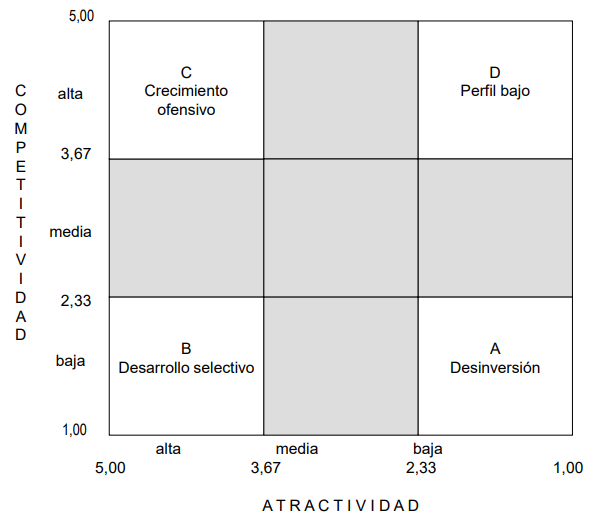
\includegraphics[width=0.4\textwidth]{img/matriz_atractivo.png}
            \end{figure}
            \item \textbf{Matriz Ciclo de vida:} Analizar el tiempo de respuesta del consumidor con respecto a un producto o servicio.
            \item \textbf{Matriz tamaño ventaja competitiva:} Análisis especifico de nuestra ventaja con respecto a otras empresas.
            \item \textbf{Matriz rentabilidad:} Comparación entre la inversion y la utilidad. 
        \end{itemize}
    \end{itemize}

\subsection{Análisis de la cadena de valor}
\begin{itemize}
    \item \textbf{Ciclo de vida}
    \begin{itemize}
        \item \textbf{Introducción:} Producto entrando en el mercado.
        \item \textbf{Aceptación:} Producto comienza a ser aceptado por el mercado objetivo.
        \item \textbf{Madurez:} Producto se estabiliza en el mercado y alcanza su punto máximo de ventas.
        \item \textbf{Saturación:} Producto comienza a perder ventas.
        \item \textbf{Obsolescencia:} Producto deja de ser vendido o el nivel de ventas llega al mínimo (Productos Perros).
    \end{itemize}
\end{itemize}

\section{Elección de estrategia}
\noindent Para elegir la estrategia a implementar, es imprescindible haber realizado previamente alguno de los análisis mencionados. Una vez completados estos análisis, las estrategias disponibles son:
\begin{itemize}
    \item Estrategia competitiva (genérica)
    \item Estrategia de crecimiento (Dinero) 
    \item Estrategia de desarrollo (Calidad de vida/productos)
\end{itemize}

\section{Negocios}
\subsection{Categoría de negocios}
\begin{itemize}
    \item \textbf{Volumen:} Alcanzar el punto preciso del mínimo costo y liderar en ventas.
    \item \textbf{Especialización:} Centrarse en un punto del mercado y ser el mejor en ese punto o cubrir todo el mercado con productos con características únicas.
    \item \textbf{Fragmentada:} Llevar a cabo varias formas de competencias, teniendo en cuenta fuerzas relativas y competencias únicas.
    \item \textbf{Estancamiento:} Sobrevivir en el mercado a través de la reducción de costos y maximización de la productividad
\end{itemize}

\subsection{Lógica de negocios}
\begin{itemize}
    \item \textbf{Lógica del cliente:} Como tener acceso a los clientes.
    \item \textbf{Lógica del producto:} Oferta diferenciada que se lleva al mercado.
    \item \textbf{Lógica económica:} Obtención de beneficios o satisfacer los criterios establecidos de beneficio económico.
    \item \textbf{Lógica estructural:} Organización necesaria para que las 3 lógicas anteriores operen en conjunto.
\end{itemize}

\begin{figure}[H]
    \centering
    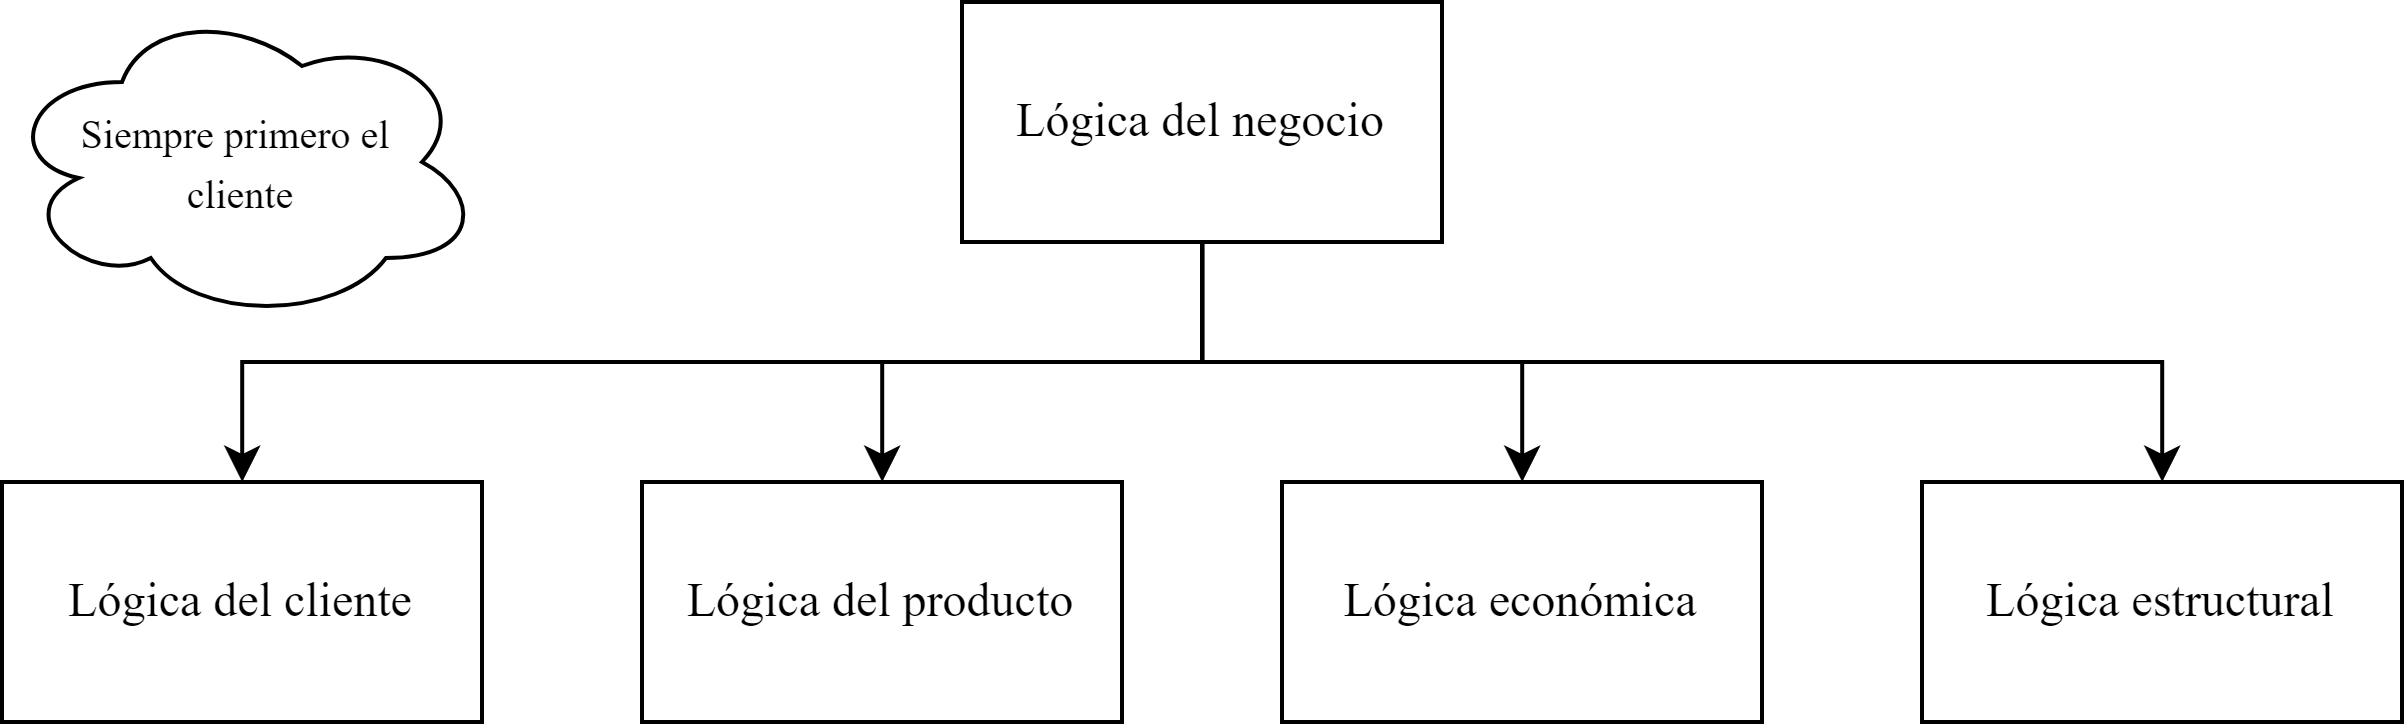
\includegraphics[width=1\textwidth]{img/logicanegocio.png}
\end{figure}

\begin{figure}[H]
    \centering
    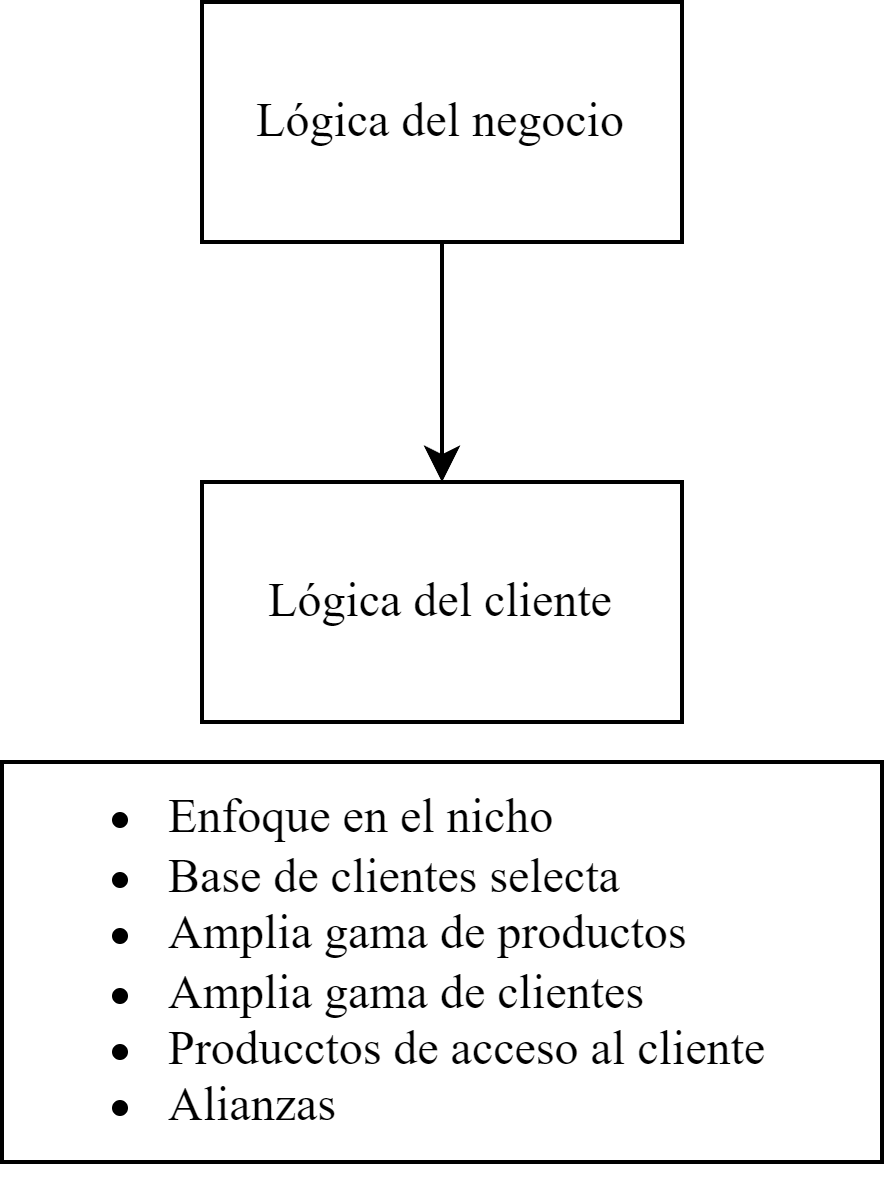
\includegraphics[width=0.45\textwidth]{img/logicacliente.png}
\end{figure}

\subsection{Cadena de valor de negocios}
\begin{figure}[H]
    \centering
    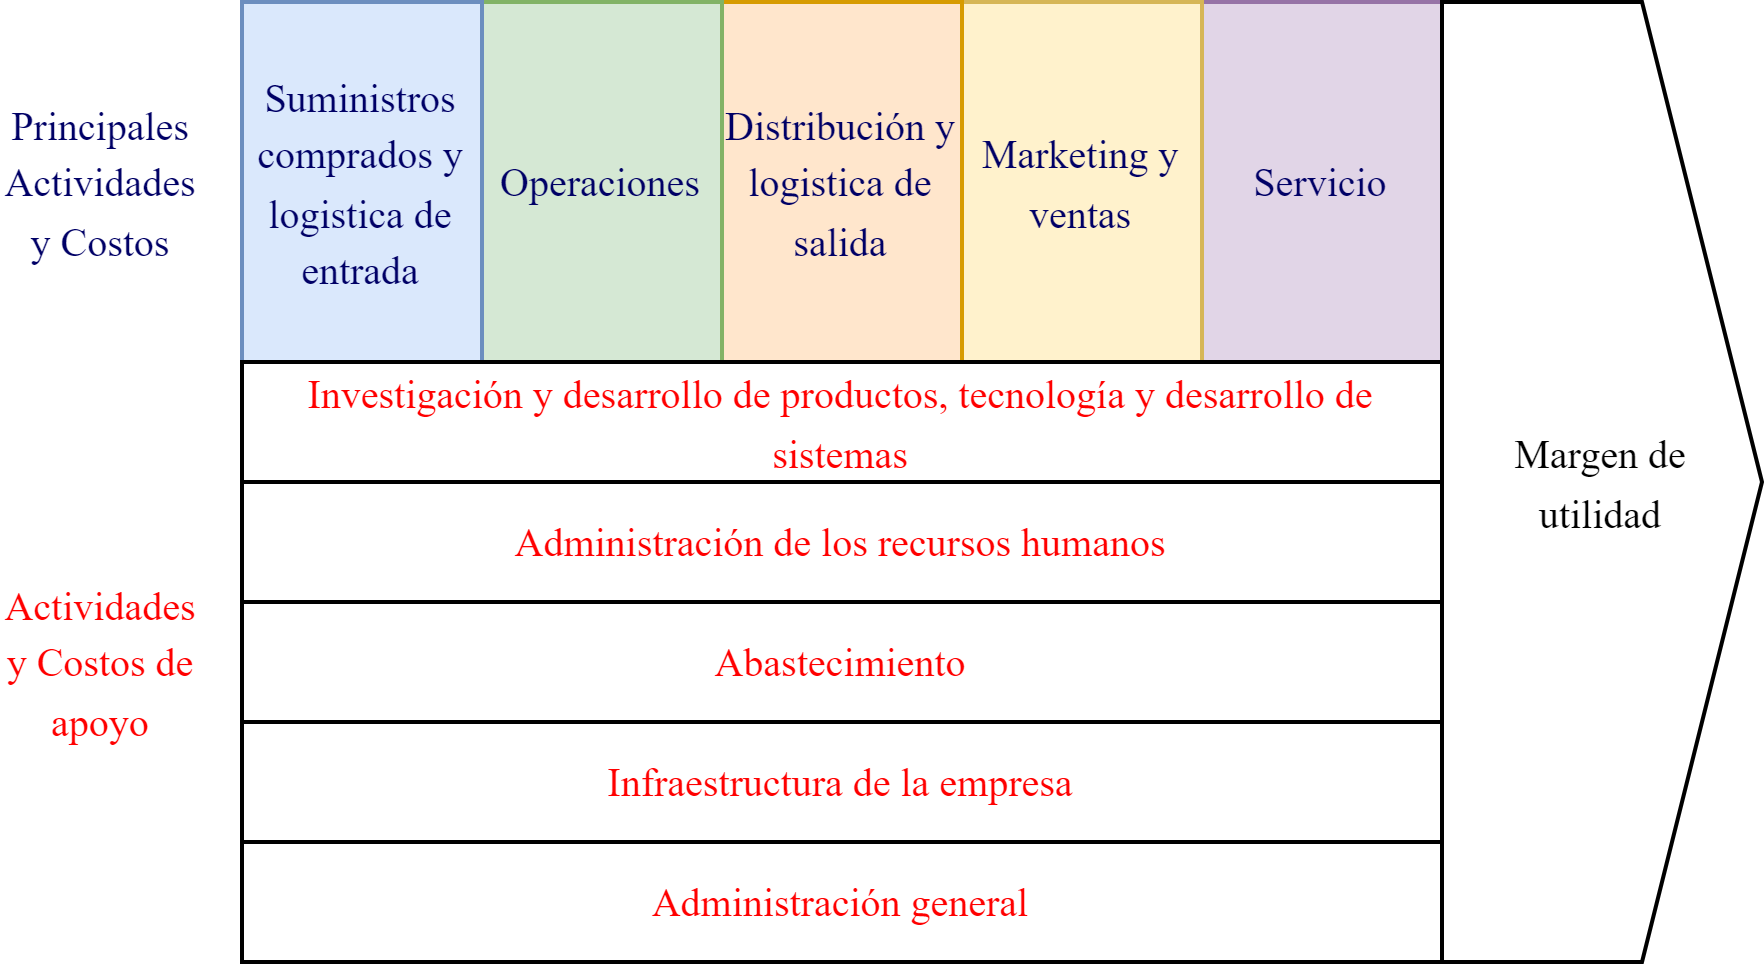
\includegraphics[width=1\textwidth]{img/costosdenoseque.png}
\end{figure}

\begin{itemize}
    \item El desglosar en este diagrama las operaciones de las actividades y procesos nos expone en gran medida los elementos que significan un costo para la empresa.
    \item Todas las actividades en la cadena de valor involucran un costo y limita activos.
    \item El asignar los costos de operación y activos a cada actividad nos permite ver un aproximado del costo respectivo.
    \item La cadena de valor y como se desempeñan las actividades reflejan la evolución del negocio, operaciones internas, estrategias, enfoques de ejecución y las economías de las actividades
\end{itemize}

\end{document}
